\documentclass[thesis.tex]{subfiles}

\chapter{Proposed Methods}
\section{BK.Synapse - A Framework for Distributed Neural Network Training}
In this section, we present a tool and framework for training neural networks in a distributed manner called BK.Synapse.

\subsection{Overview \& Motivation}
BK.Synapse provides a complete set of tools for training neural networks, including model and dataset managements, training configuration, monitoring and exporting results, combined with an intuitive, no-configuration distributed environment.

The use-cases and general design for BK.Synapse are inspired by NVIDIA DIGITS\footnote{\href{https://developer.nvidia.com/digits}{https://developer.nvidia.com/digits}} (Deep Learning GPU Training System). DIGITS' primary use case is training deep neural nets on multiple GPUs, along with several computer vision-related utilities (eg. data visualization). The tool provides an user interface for interacting with and managing datasets, models, etc,... However, there are several downsides to DIGITS' design that motivated the creation of BK.Synapse, namely:
\begin{itemize}
    \item Despite supporting Caffe, TensorFlow and LuaTorch, DIGITS' workflow is heavily optimized for Caffe. This forces major rewrites and reconfiguration for non-Caffe frameworks. For example, TensorFlow models need to be fully written within a single file, while subclassing a parent class that makes testing quite difficult.
    \item DIGITS was designed for single-machine, local deployment. This means it can only utilize multiple GPUs on the same machine, limiting scalability.
\end{itemize}

\begin{figure}[htp]
	\centering
	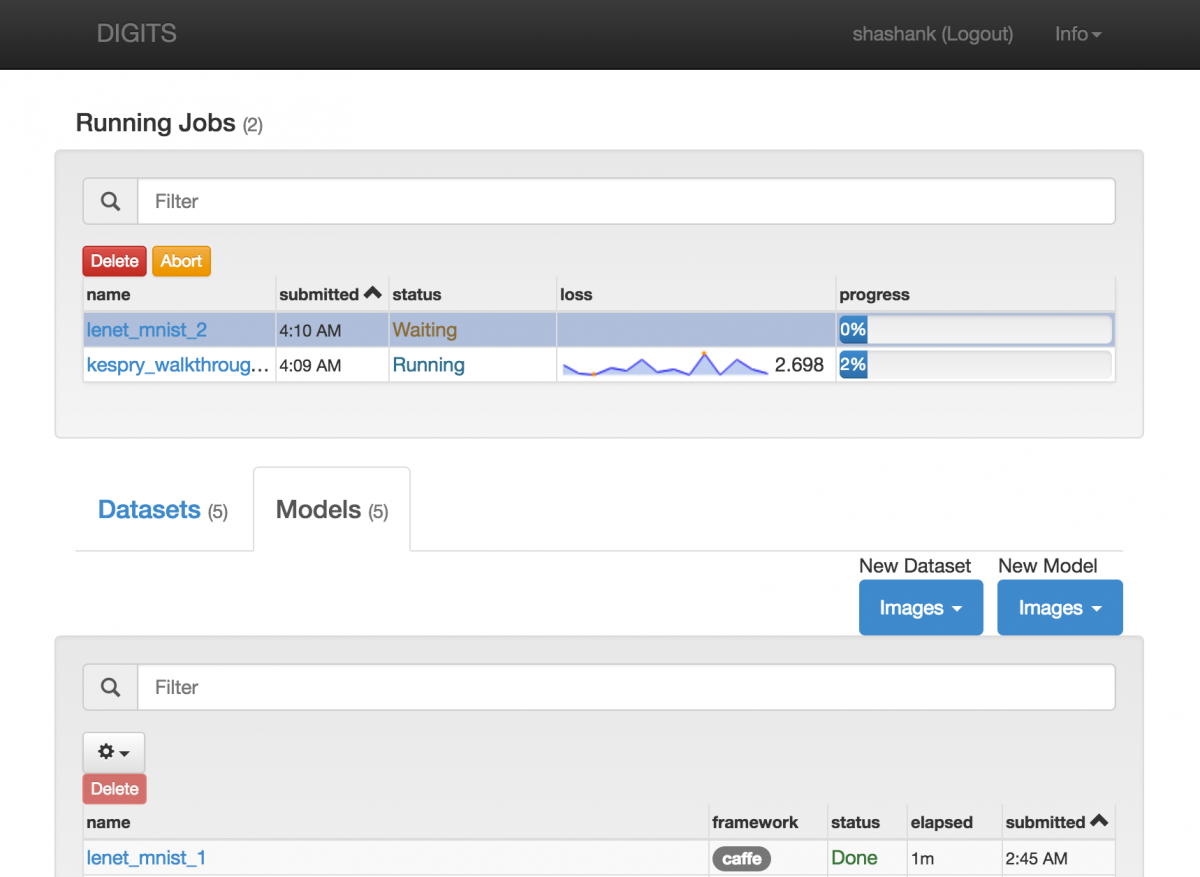
\includegraphics[width=0.7\textwidth]{digits.png}
	\caption{An example of DIGITS' user interface}
	\label{fig:digits}
\end{figure}
\FloatBarrier

Due to these limitations, we aim to design BK.Synapse as a distributed training framework with little to no development overhead. Users should be able to train networks on multiple nodes with ease, while making minimal additions to their existing codebases. With this in mind, we also target the more user-friendly PyTorch as the primary deep learning backend, with planned support for Keras and TensorFlow in the future. Table \ref{tab:digits_compare} shows a detailed comparison between BK.Synapse and DIGITS.

\begin{table}[]
\centering
\begin{tabu} to \textwidth {|l|X[c]|X[c]|}
    \hline
    \multicolumn{1}{|c|}{\textbf{Feature}} & \textbf{DIGITS} & \textbf{BK.Synapse} \\ \hline
    Single-node multi-GPU support & \cmark & \cmark \\ \hline
    Job monitoring \& management & \cmark & \cmark \\ \hline
    Open source & \cmark & \cmark \\ \hline
    Multiple node support & \xmark & \cmark \\ \hline
    Arbitrary models and datasets & \xmark & \cmark \\ \hline
    Data visualization & \cmark & \xmark \\ \hline
    Model visualization & \cmark & Partial (via Tensorboard) \\ \hline
    Backends & Caffe, TensorFlow, LuaTorch & PyTorch, Keras (planned), TensorFlow (planned) \\ \hline
\end{tabu}
\caption{Benchmark training configuration}
\label{tab:digits_compare}
\end{table}

We shall describe BK.Synapse's design and technical implementation in the following section.

\subsection{System Description}

\section{Case Study: RetinaNet for Text Region Detection}  \label{section:retinanet}
